\documentclass[aps,prc,reprint,amsmath,superscriptaddress]{revtex4-1}

\usepackage{hyperref}
\usepackage{graphicx}
\graphicspath{{fig/}}

\newcommand{\R}{\mathcal{R}}
\newcommand{\psec}[1]{\phantomsection\addcontentsline{toc}{section}{#1}}

\begin{document}

\title{Predicting outcomes in games of skill by redefining what it means to win}

\author{J.\ Scott Moreland}
\affiliation{Department of Physics, Duke University, Durham, NC 27708-0305}
\author{Matthew C.\ Superdock}
\affiliation{Department of Computer Science, Carnegie Mellon University, Pittsburgh, PA 15213}

\date{\today}


\begin{abstract}
  The Elo rating system is a highly successful ranking algorithm for games of skill where, by construction, one team wins and the other loses.
  A primary limitation of present implementations of the Elo algorithm is the ability to predict information beyond a match's win-loss probability.
  For example, in the traditional Elo system the victor is awarded the same point bounty if he beats a team by 1 point or 10 points; only the rating difference of his opponent affects the match bounty.

Previous efforts to extend the Elo system to incorporate margin-of-victory information have relied on adhoc assumptions which do not converge on the true margin dependent win probability in the relevant limits.
  In this work, we explain that Elo ratings and predictions can be naturally extended to include margin-of-victory information by simply redefining ``what it means to win''.
  We create ratings for each value of the margin-of-victory and use these ratings to predict the \emph{full} distribution of point spread outcomes for matches which have not yet been played.
\end{abstract}


\maketitle

\section{Elo rating system}

The Elo system ascribes a power ranking index $\R$ to each competitor (player or team) which can be used to predict the outcome of a future matchup.
Players with a higher rating are viewed as more likely to win their matchup, and players with a lower rating are more likely to lose.
The process is fundamentally Bayesian and rating values before and after the match reflect prior and posterior knowledge of each player's performance.

The convention is to initialize all player ratings at ${\R_0 = 1500}$, although this choice is arbitrary.
As we show momentarily, only the rating difference between two players matters, and hence the Elo rating can be initialized with any starting value.

The ratings of the competitors are then updated iteratively after each matchup.
Players gain or lose points based on the outcome of the match and the rating difference between the two competitors.
One is awarded more points for beating a stronger opponent and less points for beating a weaker opponent.
The points awarded to the victor are deducted from the loser such that the total number of points in the system is always conserved.

More specifically, the victor bounty scales with the degree to which a player exceeds (or falls short of) their expected match performance.
Let $P_\text{exp}$ denote the expected probability that a team beats their opponent at a neutral venue.
The bounties that the team and their opponent receive from the outcome of the match are given by,
\begin{align}
  \label{elo}
  \Delta \R_\text{team} &= \kappa \,(P_\text{obs} - P_\text{exp}),\\
  \Delta \R_\text{opp} &= -\Delta \R_\text{team},
\end{align}
where ${P_\text{obs}=1}$ if the team beats their opponent and ${P_\text{obs}=0}$ if the team loses, while $P_\text{obs}=0.5$ is often used if both teams tie.
The free parameter $\kappa$ modulates the relative weight of prior and posterior information. 
If $\kappa$ is small, the prior holds significant weight, and it takes many successive wins or losses to move the rating up or down.
Conversely, when $\kappa$ is large, each win or loss can significantly affect the team's rating.
Typically, the hyper-parameter $\kappa$ is tuned to optimize the veracity of model predictions by back-testing on historical games.

The expected probability $P_\text{exp}$ that a team beats their opponent is modeled using a logistic function
\begin{equation}
  \label{win_prob}
  P_\text{exp}(\R_\text{team}, \R_\text{opp}) = \frac{1}{10^{-(\R_\text{team} - \R_\text{opp})/\gamma} +1},
\end{equation}
where the free parameter $\gamma$ sets the scale of rating differences.
Much like the starting Elo, the parameter $\gamma$ can take any value and only the ratio $\kappa/\gamma$ is meaningful for observable quantities.
A common convention is to fix $\gamma=400$ such that a 400 point rating advantage corresponds to a 90\% average win rate.

A primary feature of the Elo system is that the expected win probability $P_\text{exp}$ determined from iteratively updated Elo ratings $\R_\text{team}$ and $\R_\text{opp}$, converges on the \emph{true} win probability of the matchup when the competitors sample scores from independent random variables.
In the limit of infinitely many games and infinitely small update factor $\kappa$, the Elo calculated win probability is the true win probability.
\begin{figure}
  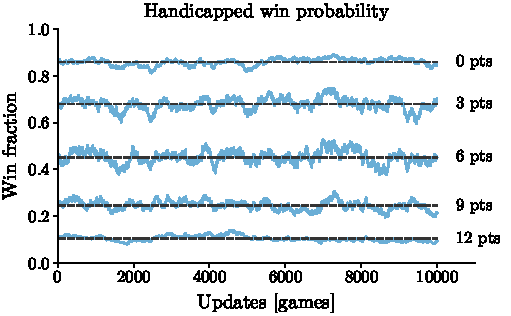
\includegraphics{win_rate}
  \caption{Time series win rate for a toy model with different handicaps (listed on the right) applied to the stronger team. The black horizontal dashed lines are the true win rate of the sampled distribution under the imposed handicap and the blue solid line is the reconstructed (predicted) win rate determined by updating handicapped and advantaged Elo ratings for each team and applying Eqn.~\eqref{win_prob_hcap}. This particular toy model is a distribution of scores sampled from the difference of two Poisson random variables. The stronger team has a mean score of $16$ and the weaker team a mean of $10$. Notice that the win rate is $\sim\!50\%$ when the handicap equals $6$ points. Actually, to be exact it is slightly below 50\% as the chosen win criteria requires that a team win by \emph{more} than 0.}
\end{figure}

\section{Margin-of-victory Elo}

The original Elo model was first applied to chess rankings where there is a winner and a loser but no score.
It can be used to predict the odds with which a player beats his opponent \eqref{win_prob}, and correspondingly---by calculating various outcomes---the odds with which a player advances through a tournament. 

The model is easily extended to point based games by ignoring the margin-of-victory and only considering wins and losses.
One shortcoming of this approach is that it cannot predict the mean or median point spreads which are often used to set betting lines and which are interesting in their own right.
Methods have been proposed to retain margin-of-victory information by allowing the parameter $\kappa$ in Eq.~\eqref{elo} to vary with the point spread.
The idea is that if a team finds itself in a rating slump, subsequent dominant victories should raise the team's rating faster than successive close wins.
The method appeared in football Elo ratings \cite{?} and was adapted to forecast NFL and NBA team performance on the analytics and news platform FiveThirtyEight \footnote{for an extensive list of Elo use cases see \ref{?}}.

Spread-dependent $\kappa$-factors possess some desirable features, but they also introduce a number of problems.
There is no obvious form for a margin-of-victory multiplier on $\kappa$, and introducing one still does not get you any closer to predicting the mean or median score of a game.
There are also issues of autocorrelation, i.e.\ great teams should not be over rewarded for winning by large margins because that's what great teams do.

There is, alternatively, a more natural extension of Elo ratings which allows one to incorporate margin-of-victory information and predict the mean and median score of future games.
We start by emphasizing that Elo ratings only require actors which compete to win games and that ``winning'' is a subjective definition itself.
Let $p_s$ and $p_a$ denote points scored and points allowed respectively.
The usual win criteria is defined as
\begin{equation}
  \text{win}: p_s - p_a > 0.
\end{equation}
This is the fair or democratic criteria as it gives each competitor a level playing field.
Just as easily, one could define winning as
\begin{equation}
  \text{win}: p_s - p_a > n,
\end{equation}
where $n$ is a finite margin-of-victory line.
This is equivalent to a normal Elo rating system where a point handicap is applied in favor of one team.

To calculate the probability that a team beats an opponent by more than $n$ points, one need only calculate the Elo ratings of the team and their opponent under an $n$-point team handicap, i.e.\ according to the win criteria
\begin{equation}
  \text{win}: p_s - p_a - n > 0.
\end{equation}
The handicapping procedure splits team ratings into two different groups: a rating handicapped by $n$ points, and a rating advantaged by $n$ points.

To get a better feel for what this does, imagine an average team under the classical Elo system which corresponds to a handicap $n=0$. 
As we apply a handicap $n$ to the home team, it becomes increasingly difficult for the team to overcome their handicap and win games.
The team's handicapped Elo rating will drop, and eventually will fall below even the worst non-handicapped team.
Simultaneously, we must also keep track of each team's performance \emph{against} handicapped teams, i.e.\ for $n \rightarrow -n$.
Naturally, this will have an opposite effect, and each team's advantaged rating will rise as their handicap goes more negative.

The procedure thus creates mirror copies of the team's rating at each value of the spread, the handicapped rating $\R_\text{team}(n)$ and advantaged rating $\R_\text{team}(-n)$.
To predict the probability that the team will beat their opponent by more than $n$ points, we apply Eqn.~\eqref{win_prob} to their handicapped and advantaged Elo ratings
\begin{equation}
  \label{win_prob_hcap}
  P_\text{exp}(\R_\text{team}(n), \R_\text{opp}(-n)) = \frac{1}{10^{-(\R_\text{team} - \R_\text{opp})/\gamma} + 1}.
\end{equation}

The procedure can easily be applied for each integer value of $n$ up to some large number in order to calculate the margin-dependent Elo ratings for every reasonable margin-of-victory.
Once done, the resulting ratings can be used to predict the probability that a team beats its opponent by any point number.
The procedure simply constructs the point spread cumulative distribution function (CDF) for the team of interest
\begin{equation}
  \label{cdf}
  F(n) = \sum_{s=n}^\infty P(s),
\end{equation}
where $s = p_s - p_a$.
This is the full probability distribution of allowable point spreads and can be used to calculate both the mean and median values.

\begin{figure*}
  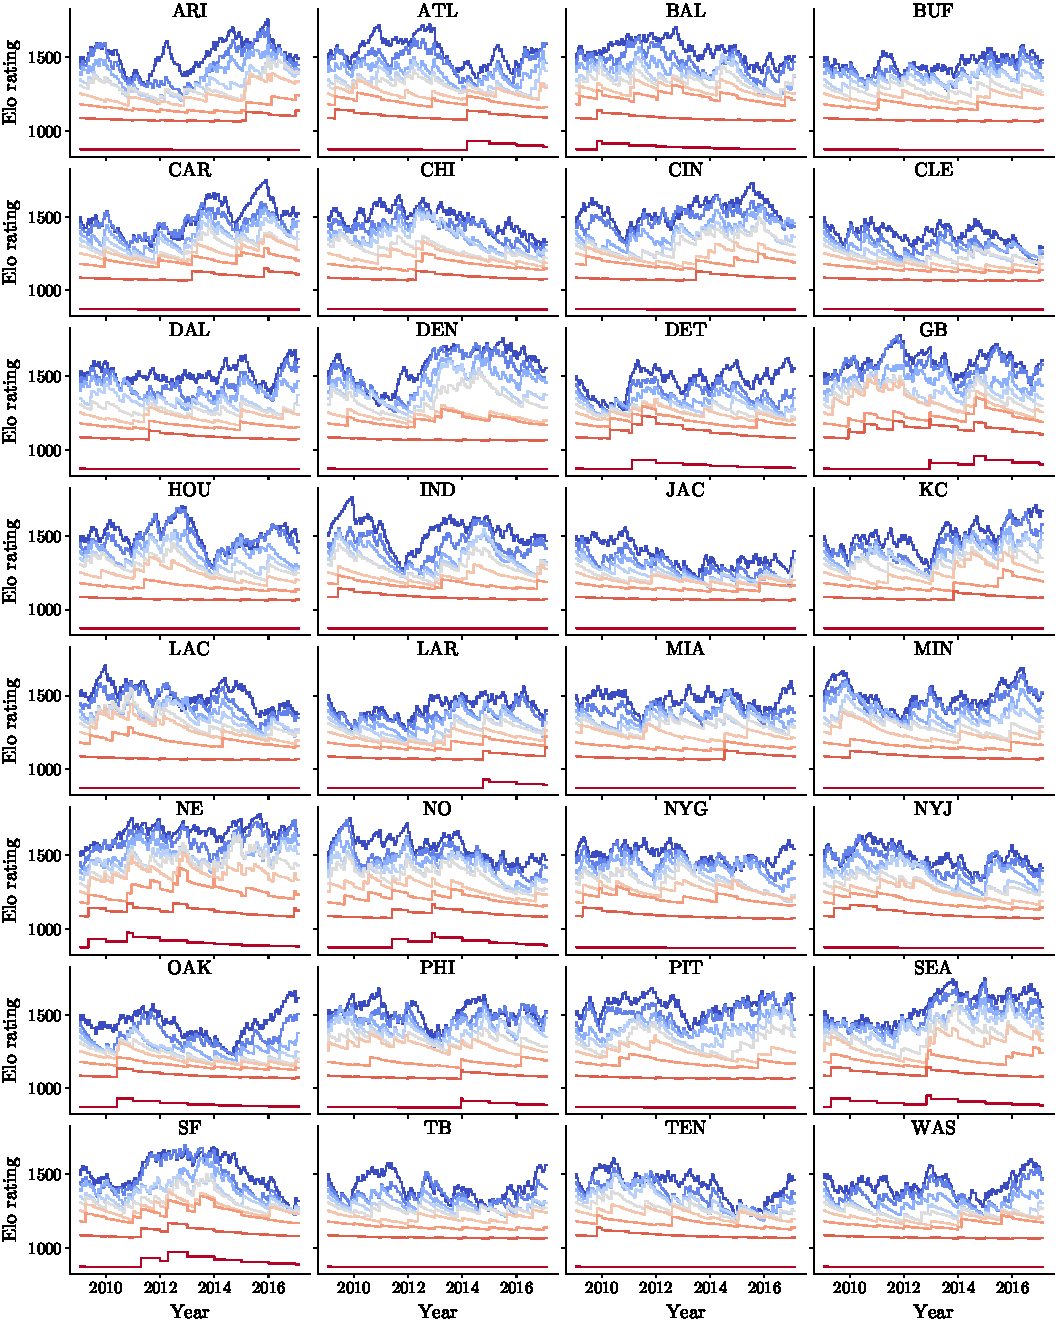
\includegraphics{team_history}
  \caption{Handicapped NFL team Elo ratings 2009--present. Colored lines denote different handicaps. Dark blue denotes a handicap of 0 points and dark red a handicap of 40 points. Intermediate colors are constant handicap increments of 5 points. Ratings for Rams and Chargers persist through relocation. Not shown: advantaged ratings which mirror handicapped ratings.}
\end{figure*}

\begin{figure}
  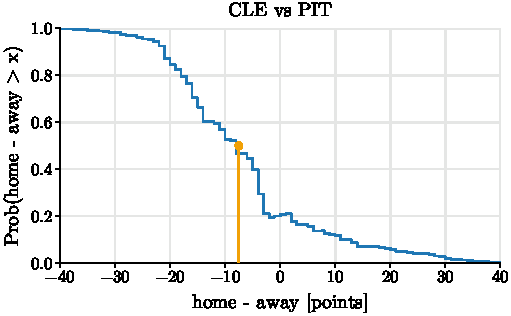
\includegraphics{example_distribution}
  \caption{Example cumulative probability distribution function (CDF) of point spreads calculated for a specific matchup from the margin-dependent Elo model. Note that the function is not strictly monotonic due to fluctuations in the decoupled Elo ratings at each value of the spread.}
\end{figure}

\begin{figure*}
  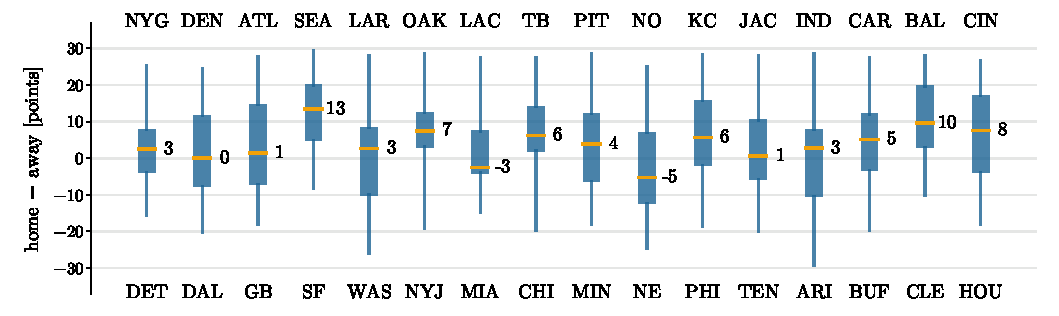
\includegraphics{paper_spreads}
  \caption{NFL score predictions determined from the margin-dependent Elo model for the second week of the 2017 season. Orange dashes are the prediction medians, boxes are the 25--75\% inner-quartile range, and whiskers cover 90\% of the distribution tails. Home field advantage was accounted for by handicapping the away team 60 Elo points.}
\end{figure*}

\section{Descriptive Statistics}

\subsection{Median point spread}

The median point spread is the value which gives both teams equal odds to cover.
It's a popular betting statistic as it generally promotes equal numbers of bets on both sides of the line which increases betting volume and minimizes risk for the house.
In the margin-dependent Elo model, we can easily estimate the median point spread by calculating the handicapped and advantaged ratings at each value of the spread, and by finding the spread where the win probability between the handicapped and advantaged teams is closest to 50\%.
This is equivalent to the point spread $\tilde{s}$ such that
\begin{equation}
  \R_\text{team}(n) \approx \R_\text{opp}(-n).
\end{equation}

One should be reasonably concerned that the handicapped Elo ratings will be unreliable for large values of the spread as the handicapped team will seldom win.
Indeed, there are large uncertainties in predicting a blowout as the statistics are simply insufficient to extrapolate from prior to future events.
In contrast to these extreme spread values, the spread median is---by definition---the value where wins and losses occur with equal probability and hence events are maximally frequent to maintain rating equilibrium.
One should expect that the median values to be relatively accurate up to the limitations of the model.

\subsection{Mean point spread}

Although the mean point spread is less commonly used in betting circles, it's nevertheless interesting to compute.
The mean point spread can be obtained from the cumulative point spread distribution $F$ via integration by parts
\begin{equation}
  \label{parts}
  \bar{s} = \sum\limits_{s_\text{min}}^{s_\text{max}} s P(s) = s_\text{max} - \sum\limits_{s_\text{min}}^{s_\text{max}} F(s),
\end{equation}
where the boundary term in Eqn.~\ref{parts} simplifies since the CDF converges to $F(s_\text{max})=0$ and $F(s_\text{min})=1$ at the extrema.

The mean and median are, in general, equal only for symmetric distributions and may differ significantly in lopsided matchups where Elo differences are large.
Such differences are particularly informative when predicting spread outcomes away from the median expectation value, e.g. when predicting a blowout. 

\section{Orthogonal point combinations}

In addition to the point spread $s = p_s - p_a$, it's also possible to predict the distribution of \emph{total} points scored $t = p_s + p_a$.
The point total and point spread values represent symmetric and asymmetric components of the two teams' point distributions and form an orthogonal basis for the joint distribution $P(p_s, p_a)$. 

Point total ratings can be constructed in an analogous fashion to the aforementioned point spread ratings, and the Elo win criteria takes a modified form
\begin{equation}
  \label{win_total}
  \text{win}: p_s + p_a - m > 0,
\end{equation}
where $m$ applies a handicap to the point total $t$.
This is equivalent to the margin-dependent spread condition, except that we've flipped the sign of the opponent's points.
In doing so, the spread difference turns into a sum, and a team wins their game if its score exceeds its opponent's \emph{negated} score by a finite margin of victory, i.e.\ if the point total of both teams exceeds a given threshold.

The procedure consequently splits each team's rating into two mirror copies as before: one rating where the team is handicapped by $m$ points and one where it is advantaged by $m$ points, i.e.\ $m \rightarrow -m$, which we label $\mathcal{R}_\text{team}(m)$ and $\mathcal{R}_\text{team}(-m)$ respectively as before.
When two teams rack up a large number of combined points, the handicapped team who's points contribute with positive weight ``wins'' the game and increases its rating while the advantaged team with the sign flipped points ``loses'' the game and decreases it's mirrored rating.
This decreases the gap between the two mirrored Elo ratings, and hence increases the probability that either team will cover the same point total in future matchups.

Elo differences are always taken between the mirrored rating pairs when predicting event probabilities such that only one sign flip enters equation \eqref{win_total}. 
Naturally, the sign flip and handicapping procedure is applied to both teams in turn such that every team carries both copies of the mirrored ratings. 

Once the point spread and point total distributions are constructed for a given game, one can predict interesting quantities such as the number of points a team will score (or allow) by taking sums and differences of the point spread and point total expectation values
\begin{align}
  \label{combinations}
  \bar{p}_s &= \tfrac{1}{2}(\bar{s} + \bar{t}), \\
  \bar{p}_a &= \tfrac{1}{2}(\bar{s} - \bar{t}).
\end{align}

In this fashion we can project offensive and defensive performances, although we caution that there is no guarantee that the linear combinations in Eqn.~\eqref{combinations} will remain positive definite which is of course required for a physical point projection.


\section{Concluding remarks}

\psec{Acknowledgements}

\medskip
The authors gratefully acknowledge use of the \href{https://github.com/BurntSushi/nfldb}{nfldb} Python package by Andrew Gallant which was used to acquire NFL game data.


\end{document}
